\documentclass[man, noapacite]{apa2}

% \usepackage{pslatex}

\usepackage[
  breaklinks=true,
  bookmarks=false,
  pdfpagelabels=false,
  hyperfootnotes=false,
  hyperindex=false,
  pageanchor=false,
]{hyperref}

\makeatletter
\let\saved@hyper@linkurl\hyper@linkurl
%\let\saved@hyper@linkfile\hyper@linkfile
\let\saved@hyper@link@\hyper@link@
\AtBeginDocument{%
  % Since the whole document is affected, only the \begin part of
  % environment `NoHyper' is needed.
  \NoHyper
  \let\hyper@linkurl\saved@hyper@linkurl % needed by \url
  %\let\hyper@linkfile\saved@hyper@linkfile % needed by \href{<file>}
  \let\hyper@link@\saved@hyper@link@ % needed by \href{<url>}
}
\makeatother


\usepackage{pdfsync}
\usepackage{apacite2}
\usepackage{amsmath}
\usepackage{graphicx}
\usepackage{topcapt}
\usepackage{color}
\usepackage{appendix}

\definecolor{DarkOrange}{RGB}{255,100,50}
\newcommand{\aen}[1]{\textcolor{DarkOrange}{[aen: #1]}}

% don't split footnotes
\interfootnotelinepenalty=10000

% comment command
\newcommand{\blue}[1]{\textcolor{blue}{#1}}

\title{Early understanding of pragmatic principles in children's judgments of negative sentences}

\author{Ann E. Nordmeyer and Michael C. Frank}
\affiliation{Department of Psychology, Stanford University}

\acknowledgements{Corresponding author: Ann E. Nordmeyer \\
Department of Psychology \\
Stanford University \\
Building 420 (Jordan Hall) \\
450 Serra Mall \\
Stanford, CA 94305 \\
Phone: 650-721-9270 \\
Email: anordmey@stanford.edu}

\shorttitle{Contexts of negation}

\abstract{Adults find negative sentences difficult to process, but an informative context can facilitate processing substantially, suggesting that much of this difficulty may come from the pragmatics of negation. Are children sensitive to the pragmatics of negation as well? Although children perform poorly on many tests of negation comprehension, we argue that these past findings are due to children's sophisticated understanding of general pragmatic principles that govern communication, rather than the conceptual difficulty of negation. In Experiment 1, replicating previous work, we found that adults rated negative sentences as more felicitous in more informative contexts.  In Experiment 2, we showed that children are also sensitive to the contexts of true negative sentences, with three- and four-year-olds also rating true negative sentences higher in more informative contexts.  We discuss children's understanding of negation and pragmatics in light of these results, arguing that the felicity of negation for both adults and children is driven by the informativeness of these sentences in context.

~\\

Keywords: Negation; Language development; Pragmatics}

\begin{document}
\maketitle


\section{Introduction}

A sentence that is both grammatical and true can nevertheless sound odd in some contexts. It would be weird to point to a banana and say ``that's not an apple,'' despite the truth of the proposition. But the same sentence becomes perfectly reasonable if the banana is sitting inside a crate of apples. Are children sensitive to the communicative principles that make the same sentence sound strange (\emph{infelicitous}) in one situation, but normal in another?

Theories of pragmatics attempt to provide an account of how language is used for communication. For example, according to Grice's \citeyear{grice1975} Cooperative Principle, speakers should produce utterances that are truthful, relevant (i.e., mention a salient feature of the physical or discourse context), and informative (i.e., effectively identify the speaker's intended referent). By assuming that speakers do so, listeners can make inferences about intended meaning that go beyond the sentence's literal meaning. Modern neo-Gricean theories tend to derive such inferences from the tension between being informative with respect to a communicative goal and minimizing the effort expended \cite{horn1984,levinson2000,frank2012}. These theories make predictions about sentence felicity: A sentence that is not relevant or informative in the given context can sound strange even when it is both grammatical and true.

In this paper, we use adults' and children's judgments of negative sentences to explore the relationship between contextual pragmatics and felicity, and to test whether children are sensitive to this relationship. Negation makes an excellent case study for understanding children's pragmatic development for two reasons. First, past work on the role of context in adults' processing of negation suggests that negative sentences are easier to process (and perhaps more felicitous) in relevant, informative contexts. Second, children fail several traditional tests of negative sentence comprehension despite producing negation in spontaneous speech at a much younger age. Below, we discuss in more depth the past work on the role of context in adults' processing of negation, and children's acquisition of negation. Finally, we describe our current experiments, which explore the effect of context on adults' and children's judgments of negative sentences, and test the hypothesis that children are sensitive to the pragmatic context of negation.

\subsection{The role of context in the processing of negation}

Negative sentences can be difficult to process, even for adults. When presented without any context, people take longer to evaluate the truth of negative sentences such as ``star isn't above plus'' compared to positive sentences \cite{hclark1972, carpenter1975, just1971, just1976}. In EEG studies, participants who read true negative sentences like ``A bird is not a truck'' show an N400 response (a negative waveform that responds to semantically unexpected stimuli) similar to corresponding false positive sentences like ``A bird is a truck'' \cite{fischler1983, ludtke2008}. Based on these findings, it has been suggested that there is something specific to the representation of negation that makes processing negative sentences so challenging.

As our original example demonstrates, however, negative sentences are particularly sensitive to the effects of context.  In a classic study, \citeA{wason1965} found that when participants were asked to describe an array of seven red dots and one blue dot, participants who described the stimuli in terms of an exception to a rule (e.g., ``Circle number four is blue and the rest are red'') were faster to process true negative sentences such as ``Circle four is not red'' compared to participants who described the stimuli in other ways (e.g., ``Seven circles are red and one is blue''). Similarly, supportive written contexts, such as a narrative framing where the negated feature is made salient prior to reading the negative sentence, can facilitate the processing of negation \cite{glenberg1999, ludtke2006, nieuwland2008, dale2011}. In event-related potential studies, these contexts have also been shown to reduce the N400 response (a marker of semantic unpredictability) for true negative sentences \cite{nieuwland2008}.

Although these findings suggest that context can have a powerful effect on the processing of negative sentences, it is not clear what mechanism leads to this facilitative effect. One possible mechanism is that unsupportive contexts make negative sentences difficult because they are pragmatically uninformative. In recent work (\citeNP{nordmeyer2014}; Nordmeyer \& Frank, under review), we demonstrated a graded effect of context on the processing of negation, with negative sentences processed faster as the base rate of the negated feature increased. Specifically, negative sentences that were more relevant and informative given the context were processed faster. We found that this effect of context could be reliably predicted by the probability of a speaker using the same sentence to describe the same picture. Speakers are unlikely to produce sentences that are uninformative and irrelevant, and correspondingly listeners take longer to respond to unlikely sentences.

In the current paper we explore whether children show an explicit awareness of the pragmatics of negative sentences by examining their felicity ratings in response to negative sentences in pragmatically supported vs. unsupported contexts. If children, as well as adults, rate negative sentences as more felicitous in pragmatically supported contexts, this suggests that the processing and comprehension difficulties associated with negative sentences can be explained by general pragmatic principles. We propose that children's apparent difficulty with negation is in fact due to their sensitivity to these same pragmatic principles rather than an undeveloped semantic understanding of negation or a processing difficulty that is specific to negation. In the next section, we discuss children's difficulties with negative sentences and consider a possible pragmatic explanation for children's behavior.

\subsection{Children's understanding of negation}

Although children begin producing negation spontaneously and accurately before age two \cite{bloom1970, pea1980, pea1982}, preschoolers struggle to respond correctly to true negative sentences. For example, the majority of three-year-olds and nearly half of four- and five-year-olds classified true negative sentences as ``wrong'' when an experimenter pointed to an apple and said ``this is not a banana'' \cite{kim1985}, even though they had no difficultly classifying true and false positive sentences.  This finding, along with others \cite{gilkerson2002, loder2006, nordmeyer2014b}, suggests that children struggle to process negative sentences, despite the fact that they produce them so early.

There are several reasons why children may struggle to comprehend negative sentences. One possibility is that young children do not have a fully developed semantic understanding of words like ``no'' and ``not.'' Some functions of negation, such as refusal (e.g., ``no go outside'' to express a desire to stay indoors), are produced earlier than denial/truth-functional negation, which requires evaluating a proposition to determine its truth value. Children who fail comprehension tests of denial negation may not fully understand the semantics of negation, or may not have the cognitive abilities to evaluate the truth of a proposition. Conceptual differences in types of negation also covary with syntactic differences, at least in English \cite<see>{cameron-faulkner2007}. For example, clear expression of denial negation often requires the use of ``not'' in a complex syntactic frame (e.g., ``Nathaniel's not a king'', \citeNP{drozd1995}). In contrast, rejection can easily be expressed in a single-word utterance (``'no!''). This covariation further complicates inferences about the sources of developmental differences. Thus, children's difficulty comprehending negative sentences could reflect a genuine failure to understand the semantics and/or the syntax of negation.

Another possible solution to this puzzle, however, is that children's behavior is influenced by the pragmatics of the communicative situations that they are in.  In most experiments on children's comprehension of negation, such as the one described above, children hear negative sentences without any supportive pragmatic context. In these contexts, although the sentences are not \emph{false}, they are perhaps \emph{wrong} according the the Cooperative Principle. In contrast, studies that have elicited spontaneous negations from children tend to use familiar contexts, such as reading picture books in an interactive, game-like setting \cite{pea1982, hummer1993, austin2014}. When children hear a true negative sentence and indicate that it is ``wrong'' \cite<e.g., >{kim1985}, they may be reacting to the infelicity of the sentence rather than its truth value.

There is some evidence that children's comprehension of negation is sensitive to contextual differences, similar to work on adults' processing of negation (\citeNP{devilliers1974}, see \citeNP{gualmini2004} for further discussion). In a child-friendly adaptation of \citeA{wason1965}, \citeA{devilliers1974} found that children were faster and less error-prone to complete a sentence such as ``This is not a $\rule{2cm}{0.15mm}$'' when the experimenter pointed to an object that was an exception in a set of objects (i.e., pointing to a cow amongst six horses). While this study does suggest that children are sensitive to the contexts of negation, it does not tell us whether children's apparent failure to comprehend negative sentences in unlicensed contexts (i.e., \citeNP{kim1985}) is due to an awareness of the relative (in)felicity of negation in certain contexts rather than a true failure to comprehend the negative element. Examining children's explicit felicity judgments to negative sentences in different contexts, rather than relying on implicit measures, can help us understand why and how context might play a role in children's comprehension of negation. 

If the effect of context on negation is primarily pragmatic in nature, we can use negation as a case study to explore children's sensitivity to contextual pragmatics. Evidence is mixed regarding whether children are sensitive to Gricean pragmatic principles. Some data suggest that children struggle to compute scalar implicatures; for example, accepting a sentence like ``Some of the horses jumped over the fence'' in a scenario where \emph{all} of the horses had jumped over the fence (\citeNP{papafragou2003}, see also \citeNP{noveck2001}). Other evidence, however, suggests that children are sensitive to pragmatics and can make a number of pragmatic inferences about contextually-based implicatures \cite{papafragou2004, barner2011, yoon2015, stiller2015}, adjective use \cite{horowitz2012, horowitz2015}, and epistemic states \cite{hochstein2014}. 

By examining children's explicit judgments of negative sentences in different contexts, we can ask whether children's difficulty with negation is actually due to their sensitivity to pragmatics. When children say that a true negative sentence is ``wrong,'' they may be commenting on the felicity of the sentence rather than the truth value, demonstrating awareness that the same sentence can be a ``good'' thing to say in one context but a ``silly'' thing to say in another. We hypothesize that children's apparent late comprehension  of negation in laboratory investigations is driven by the same pragmatic mechanisms that make negation appear to be challenging for adults.

\subsection{The current studies}

In this work we investigate how adults' and children's explicit felicity judgments of negative sentences are influenced by the contexts in which those sentences appear. We operationalize context as information that influences expectations about an upcoming utterance.  In natural contexts, the information that constitutes ``context'' could include visual information, words, or actions in the setting of a conversation or another shared task \cite{clark1996}. In our experiments, we use visual contexts in which we manipulate the base rate of certain features in the stimuli. For example, in a context where three people have apples and one person does not, it feels very natural to describe the last person by saying ``He doesn't have an apple.'' In contrast, in a context where no one is holding any objects (i.e., there are no apples present anywhere), the same sentence is uninformative, because it could refer to any of the people in the scene and there is no reason to discuss apples.

First, we explore adults' judgments of negative sentences to confirm that adults prefer negative sentences in more informative contexts, supporting the findings of past research in the domain of sentence processing \cite<e.g.,>{nordmeyer2014}. We then examine whether preschoolers' sentence judgments are also sensitive to the contexts of negative sentences. If children's difficulty comprehending negative sentences is due to conceptual complexity or an undeveloped semantic understanding of negation, then these children should rate true negative sentences as being bad in any context. If, however, children are actually rating true negative sentences as ``wrong'' because of the infelicity of pragmatically unsupported negation, then we should see children's performance improve when they are asked to rate true negative sentences in a supportive, informative context. We find evidence for the latter hypothesis, suggesting that when children rate pragmatically unsupported negative sentences as ``bad'' in classic tests of negation, they are explicitly reacting to the felicity of those sentences rather than failing to process the negation. 

%We hypothesize that the effects of context on the felicity of negative sentences is driven primarily by Neo-Gricean pragmatic principles. To formalize this prediction, we compare the results of our adult data in Experiments 1 and 2 to the predictions of a Rational Speech Act model \cite{frank2012}, which predicts that listeners expect speakers to produce maximally informative utterances. In the above examples, the RSA model predicts that the sentence ``he doesn't have apples'' is more informative (and therefore more likely to be produced) in the context where everyone else has apples, because in this context the utterance uniquely identifies the referent of the sentence. We find that sentences that are more probable according to this model are rated as more felicitous by our participants.

%\aen{move this???} In sum, the results of past research on negation suggest a paradox: Negative sentences are produced early by children and frequently throughout adulthood, yet both adults and children appear to find negation difficult on tasks that test their processing and comprehension. Our data suggest that the difficulty of negative sentences is due primarily to the infelicity of negative sentences in unsupported contexts, rather than any representational or syntactic difficulty specific to negation. Negative sentences are more likely to violate the Cooperative Principle, because a negative sentence can refer truthfully to a broader set of referents (e.g., at any given moment, there are more people in the world who are \emph{not} holding apples than people who \emph{are} holding apples, more boxes that do \emph{not} contain chocolate than boxes that \emph{do} contain chocolate, etc.), making negative sentences less informative by default. In the right contexts, however, negative sentences can be just as informative as positive sentences, suggesting that the ``difficulty'' of negation is actually due to a general difficulty understanding unlikely (and therefore infelicitous) utterances.

\section{Experiment 1}

Past work on adults' processing of negation suggests that negative sentences are easier to process in more informative contexts \cite<e.g.>{nordmeyer2014}. In Experiment 1, we extend these findings to explicit felicity judgments. This experiment had two goals, first to replicate previous findings with adults using a felicity measure, and second, to ensure that the stimuli in our developmental experiment produced strong judgments with adults.

Half of the participants in Experiment 1 saw sentences presented in a context where none of the surrounding characters had any objects on their table (the none context), and the other half saw sentences presented in a context where everyone except for the target character possessed the negated object, e.g., apples (the target context). Our prediction, based on Neo-Gricean pragmatic principles and past findings, was that adults would rate negative sentences as more felicitous in the target context, because the negation is more informative (i.e. uniquely selects the intended referent) in this context.

In addition to context, we explored two additional factors that might influence adults' felicity judgments (and hence, whose measurements would allow us to tailor our developmental experiment). The first was referent type. The same negative sentence can refer to the absence of a feature (nonexistence) or to an alternative feature (alternative). For example, the sentence ``This box doesn't contain apples'' might refer to an empty box (i.e., nonexistence) or a box containing an alternative object (e.g., bananas instead of apples). Previous work suggests that adults are faster to identify the referent of nonexistence compared with alternative negation \cite{nordmeyer2013, nordmeyer2014b}. This finding could be due to processing demands: Identifying a missing feature is easier than identifying a changed feature. It could also reflect an expectation about the pragmatics of negation, however; adults may find alternative negation infelicitous because they expect the sentence to describe present, rather than absent, features. In Experiment 1, half of the true negative trials referred to a character who had nothing (nonexistence negation) and half of true negative trials referred to a character who had some other object, e.g., a cat (alternative negation).

The second factor we varied was the syntactic framing of negation (e.g., ``has no apple'' and ``doesn't have an apple''). Certain types of negation are often produced in particular syntactic frames; thus, it might be more natural to express denial negation using the ``doesn't have'' frame. On the other hand, if the facilitative effect of context on negation is driven by the informativeness of negative sentences in different contexts, then these same effects should appear regardless of the syntactic framing of the sentences.

\subsection{Method}

\subsubsection{Participants}

We recruited a planned sample of 100 adults to participate in an online experiment through Amazon Mechanical Turk; six participants were excluded for indicating that they were under 18 after completing the experiment, and two participants who did not list English as their native language were excluded. Of the remaining 92 participants, 49 were male and 40 were female, three declined to report gender, and ages ranged from 18 -- 65+. We restricted participation to individuals in the United States and paid 35 cents for the experiment, which took approximately five minutes to complete. Participants were randomly assigned to either the none context (n=47) or the target context (n=45).

\subsubsection{Stimuli}

We created 16 trial items. On each trial, four Sesame Street characters were shown standing behind tables. One character was randomly selected as the ``target'' character, designated by a red box (see Figure \ref{fig:trial}). The remaining three characters were designated as ``context'' characters.


\begin{figure}[t]
\begin{center}
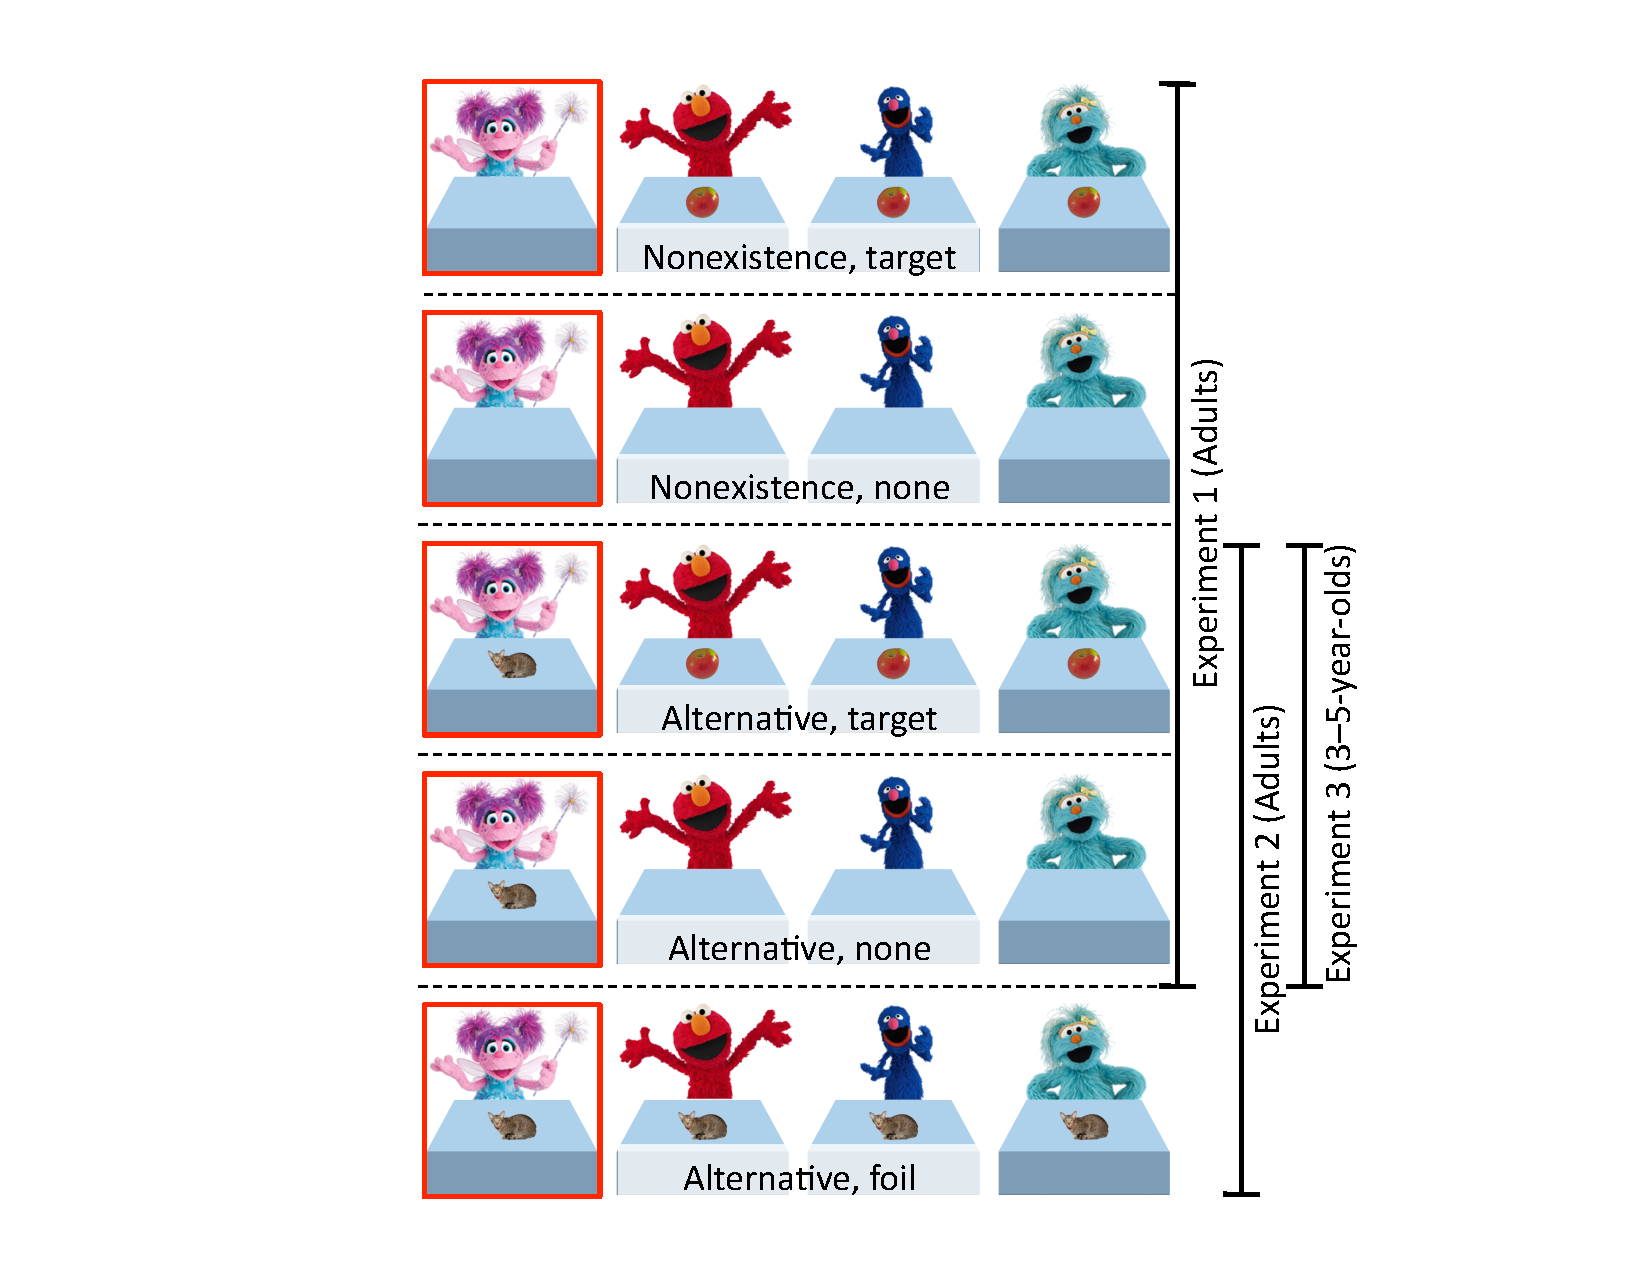
\includegraphics[width=4.5in]{figures/trialtypes.pdf}
\caption{\label{fig:trial} The four types of true negative trials across Experiments 1 and 2. In this example, the target object is an apple and the alternative object is a cat. Below each set of pictures a sentence appeared about the character in red, e.g., ``Abby doesn't have an apple.'' }
\end{center}
\end{figure}

In the none context, the context characters all stood behind empty tables. In the target context, each context character had an identical object on their table. The objects belonged to one of four categories: animals (cat, dog, horse cow), vehicles (car, bus, boat, truck), food (apple, banana, cookie, orange), and household objects (fork, spoon, bowl, plate). Stimuli were created using images from the Bank of Standardized Stimuli \cite{brodeur2010}.

Below the characters was a sentence about the target character. Across the entire experiment, six of these sentences were positive sentences such as ``[character] has a/an [object].'' Five were negative sentences of the form ``[character] has no [object]'' and five were negative sentences of the form ``[character] doesn't have a/an [object].''

The target character had a target object, an alternative object (``alternative'' trials), or nothing (``nonexistence'' trials), allowing us to examine two different negative concepts (see Figure \ref{fig:trial} for depictions of these trials and the different context conditions).  Trial conditions were crossed such that each participant saw six true positive trials, two false positive trials (one alternative and one nonexistence), two false negative trials (one ``has no'' sentence type and one ``doesn't have'' sentence type), and eight true negative trials (two ``has no''/nonexistence, two ``has no''/alternative, two ``doesn't have/nonexistence,'' and two ``doesn't have/alternative''). Each of these trial types was randomly assigned to a target object, and trials were presented in a random order.

A slider bar was positioned beneath the sentence, with a seven-point scale ranging from ``Very Bad'' to ``Very Good.'' A progress bar at the top of the screen informed participants how much of the experiment they had completed.

\subsubsection{Procedure}

Participants first saw an instructions screen that briefly described the task and informed them that they could stop at any time. Once participants agreed to participate, they saw an instructions screen that explained the task in more detail. On each trial the pictures, sentence, and a slider bar to indicate sentence judgment appeared simultaneously. Participants had to make a selection on the sliding scale in order to progress to the next trial. Participants were encouraged to use the entire scale.\footnote{The experiment can be viewed at \href{http://anordmey.github.io/neg-tablet/experiments/exp1/negadult.html}{\nolinkurl{http://anordmey.github.io/neg-tablet/experiments/exp1/negadult.html}}}.

When using the ratings scale to make judgments about sentences, participants were asked to rate how ``good'' each sentence was based on how a hypothetical speaker might behave, e.g., ``if no one would ever say a particular sentence in this context, or if it is just wrong, rank that as `Very Bad,' but if something is right and sounds perfectly normal, mark it as `Very Good.'''  This resulted in a scale where the bottom end of the scale (`Very Bad,', `Bad', etc.) could be used for sentences that are blatantly false, as well as sentences that are true but pragmatically infelicitous. This was a deliberate choice based on our interest in children's responses to these sentences. On past sentence judgment tasks, children often say that true negative sentences are ``wrong'' \cite<e.g.,>{kim1985}. Our hypothesis is that children are judging the felicity of the sentence as well as the truth value on these tasks. Because we believed that children were already treating the scale this way, and we were concerned that having two separate rating scales would be too complex for children, we chose to explicitly conflate felicity and truth value in both our adult and child experiments.

\subsection{Results and Discussion}

Participants treated the scale as expected, consistently rating true sentences much higher than false sentences.  Furthermore, participants consistently rated positive sentences higher than negative sentences. There was no effect of context, syntactic frame, or referent type on true positive sentences, false positive sentences, or false negative sentences, likely due to a ceiling effect for true positive sentences and a floor effect for false sentences (see Appendix A).


\begin{figure}
\begin{center}
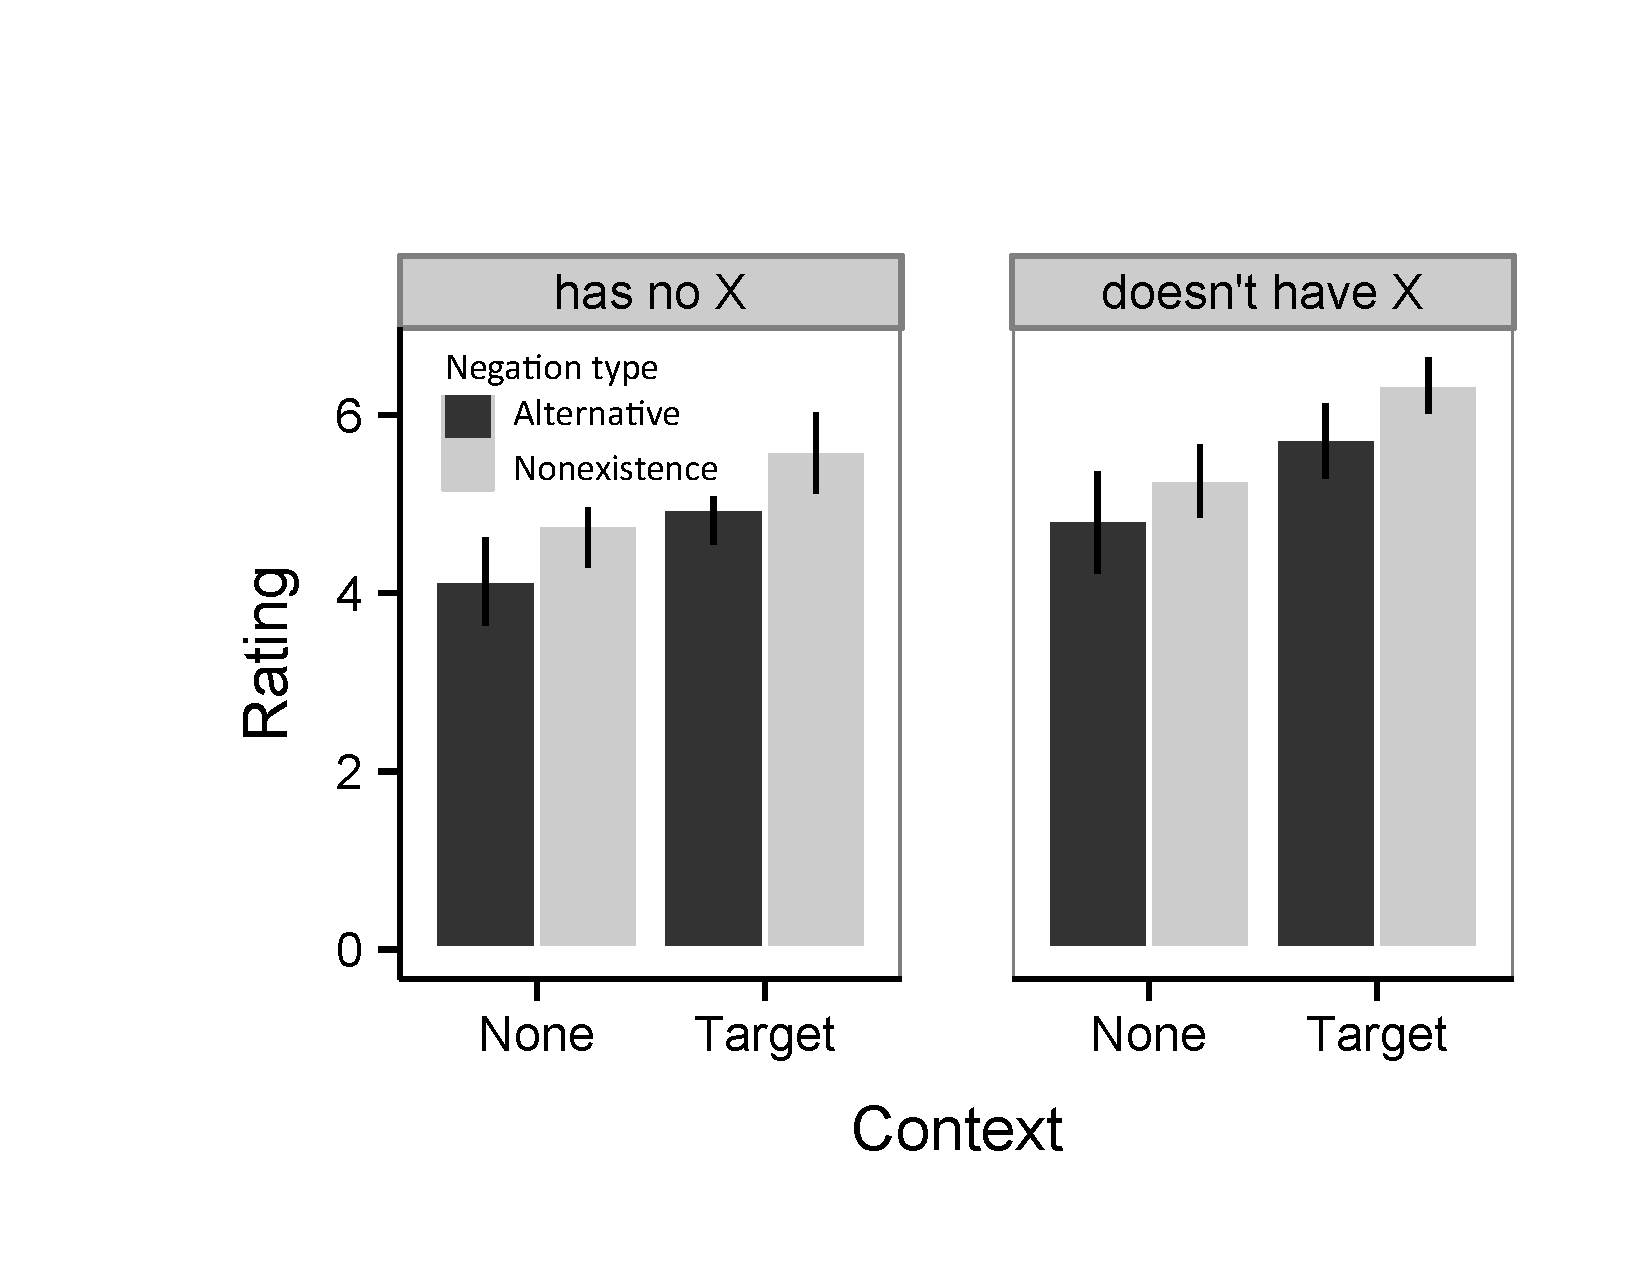
\includegraphics[width=4in]{figures/study1.pdf}
\caption{\label{fig:s1} Ratings for different types of true negative sentences in Experiment 1. Sentences of the form ``...has no X'' are shown on the left, and sentences of the form ``...doesn't have X'' are shown on the right. Trials with a none context are shown in black, and trials with a target context are shown in gray. Error bars show 95\% confidence intervals.}
\end{center}
\end{figure}

We focused our primary analysis on true negative sentences, because true negative sentences are the most challenging sentence type in classic sentence verification tasks \cite<e.g., >{hclark1972} and show the strongest context effects in sentence processing tasks \cite<e.g., >{nieuwland2008, nordmeyer2014}. As we predicted, these sentences were rated significantly higher in a target context compared to a none context. For example, the sentence ``Abby has no apple'' was rated higher when all of the other characters \emph{had} apples, compared to contexts where all of the other characters had nothing. This finding supports our hypotheses and replicates patterns previously seen in studies of processing time using explicit felicity judgments. Negative sentences expressing nonexistence were rated as more felicitous than negative sentences referring to an alternative object (see Figure \ref{fig:s1}).

To assess the reliability of these findings, we fit a linear mixed-effects model examining the interaction between context, referent type (e.g., nonexistence or alternative), and negation framing (e.g., ``has no X'' vs. ``doesn't have X'') on felicity ratings.\footnote{The model specification was as follows: \texttt{rating $\sim$ context~$\times$~referent type~$\times$~negation frame + (referent type~$\times$~negation frame~\textbar~subject) + (referent type~$\times$~negation frame~\textbar~item)}. All categorical variables were deviation coded. Significance was calculated using the standard normal approximation to the $t$ distribution \cite{barr2013}. Data and analysis code can be found at \href{http://github.com/anordmey/neg-tablet}{\nolinkurl{http://github.com/anordmey/neg-tablet}}.} Because we were primarily interested in the effects of context on true negative sentences, we focused on these trials in our analyses, though the effects reported here are significant in full models of all sentence types as well.

Examining the model, we found a main effect of context, with true negative sentences presented in a none context eliciting significantly lower ratings than true negative sentences presented in a target context ($\beta= -0.90$, $p< .001$). We found a main effect of referent type, with alternative negation receiving significantly lower ratings than nonexistence negation ($\beta= -0.60$, $p< .001$), as well as a significant effect of negation framing, with sentences of the form ``has no X'' receiving lower ratings than sentences of the form ``doesn't have X'' ($\beta= .71$, $p< .01$). There were no significant interactions between negation frame, referent type, and context.

Participants rated negative sentences with the framing ``doesn't have an X'' higher than sentences with the frame ``has no X.'' This finding might reflect an overall expectation for denial negation to be expressed using the ``doesn't have an X'' frame. This preference did not interact with context or referent type, however; participants preferred the ``doesn't have'' framing for both alternative negation and nonexistence negation, and rated both sentence frames higher when they were presented in a target context. This finding suggests that effects of context on the felicity of negative sentences are not due to features of a specific syntactic frame.

In previous work we found that adults were somewhat faster to look at the referent of nonexistence negation compared with alternative negation \cite{nordmeyer2014b}. In that experiment, the difference between nonexistence and alternative negation could have arisen because of superficial, stimulus-level differences (i.e., it might be easier to identify a character with nothing than one with an alternative object). Our replication of this result using explicit felicity judgments suggests that this difference may be due to pragmatic factors as well. One explanation for participants' preference for nonexistence negation is that a sentence such as ``Abby doesn't have an apple'' is more informative when Abby has nothing compared to when she has an alternative object. In a strong context (e.g., one where everyone else has apples), using negation to point out Abby's lack of apples is informative because it uniquely identifies her character in the array. When Abby has some alternative object (e.g., a cat), however, there is a \emph{more} informative utterance that a speaker could use (e.g., ``Abby has a cat''). The existence of a more informative utterance makes these negative sentences less felicitous, even when they appear in context.

Overall, we found that a pragmatic context increases the felicity judgments of negative sentences. Across all types of negation, participants assigned higher ratings to sentences that were presented with a target context compared to sentences that were presented with a none context. This corroborates previous work in which more informative negative sentences were processed faster than less informative negative sentences \cite{nordmeyer2014}.

\begin{table}[t]
\caption{\label{tab:s1} Coefficient estimates from a mixed-effects model predicting true negative sentence ratings in Experiment 1.}
\begin{center}
\small\addtolength{\tabcolsep}{-5pt}
\begin{tabular}{rrrr}
 \hline
 & Coefficient & Std. err. & t value \\
 \hline
(Intercept) & 5.21 & 0.13 & 38.78 \\
 Context & -0.90 & 0.33 & -3.45 \\
 Referent type & -0.60 & 0.12 & -5.05 \\
 Frame & -0.68 & 0.17 & -3.99 \\
 Context $\times$ Referent type & 0.11 & 0.19 & 0.55 \\
 Context $\times$Frame & 0.15 & 0.29 & 0.52 \\
 Referent type$\times$Frame & -0.11 & 0.18 & -0.64 \\
 Context$\times$Referent type$\times$Frame & -0.22 & 0.32 & 0.67 \\
  \hline
\end{tabular}
\end{center}
\end{table}

\section{Experiment 2}

In Experiment 2, we examine whether children, like adults, are more likely to find a negative sentence felicitous in an informative context. Past work suggests that children produce negation very early \cite{bloom1970, pea1980}, but struggle on classic comprehension tasks for several more years \cite<e.g., >{kim1985}. Children's success in these tasks varies with the context that a negative sentence occurs in \cite<e.g., >{devilliers1975, nordmeyer2014b}, which could explain this apparent gap between production and comprehension. If children expect speakers to produce informative utterances, then on classic comprehension tasks they might be reacting to the infelicity of a negative sentence without context rather than its truth value. Under this account, children should perform differently when they are asked to evaluate negative sentences in a supportive context.

To simplify the experiment for children, we focused on alternative negation in a single sentence frame, and used a between-subjects design.\footnote{A between-subjects design was chosen instead of the within-subjects design of Experiment 1 due to concerns about the length of the study. Pilot testing suggested that most children would not have tolerated a longer experiment, and adding an additional context factor would have left us with very few trials of each type. For the same reason, we only tested children on alternative negation and not nonexistence negation; see general discussion for discussion of differences in children's processing of alternative and nonexistence negation.} Based on its higher overall felicity in Experiment 1, we selected the sentence framing ``[character] doesn't have a/an [object]'' for all trials. Children were introduced to a puppet who was ``just learning how to talk, and sometimes makes mistakes,'' and were asked to help the puppet learn by indicating on a 5-point smiley face scale whether the puppet's sentence was ``good'' or ``silly or a mistake.'' Children indicated their choice by selecting the face that corresponded to their choice on an iPad \cite<for a discussion of using tablets to collect data from children, see>{frankinpress}. We deliberately conflated felicity (i.e., ``silliness'') and truth value in order to encourage children to use the negative side of the scale for both incorrect sentences as well as silly sentences. In past studies using similar paradigms \cite<i.e., >{kim1985}, children treated true negative sentences as ``wrong;'' here we evaluate if children are in fact reacting to the (in)felicity of these sentences by comparing their performance in infelicitous contexts (the none context) to their performance in felicitous contexts (the target context).

\subsection{Method}

\subsubsection{Participants}

Families visiting Children's Discovery Museum (CDM) in San Jose, CA were invited to participate in this study. Because our mission at CDM is to recruit a diverse sample of families, we used preset criteria for inclusion in the final sample but recruited inclusively regardless of language background. We also recruited from a broad range of ages, setting a target of 32 children included per age group (three- and four-year-olds) and ending data collection once this minimum had been reached in all groups after the rejection criteria were applied. In exchange for participation, children were given a sticker and a certificate.

Children who failed to understand the scale---based on their performance on positive sentences---were rejected from the analysis. Children's responses to true positive sentences were coded as correct if they chose a happy face on the scale (4 or 5), and children's responses to false positive sentences were coded as correct if they chose a sad face on the scale (1 or 2). Children who chose an incorrect response on more than 2 trials were rejected from analysis. Eight children were rejected based on this criteria, four three-year-olds and four four-year-olds. These exclusions resulted in a final sample of 69 children whose data was analyzed: 35 three-year-olds (mean age = 3;7, range = 3;0 -- 3;11, 20 female and fifteen male) and 34 four-year-olds (mean age = 4;5, range = 4;0 -- 4;11, 17 female and 17 male).

Additional children were run but not included in the final sample based on preset criteria. Fourteen were excluded for being outside the target age range (between three and five years old). Sixteen children were excluded based on having parents who indicated that they were exposed to English less than 75\% of the time. One child was excluded for parental interference during the task. Twelve children declined to continue the experiment after going through the instructions and practice trials, and five additional children were excluded for completing fewer than half of the trials.

\subsubsection{Stimuli}

Trials in Experiment 2 had the same structure as trials in the alternative/target and alternative/none contexts of Experiment 1 (see \ref{fig:trial}), but with only 16 trials. All negative sentences were of the form ``[character] doesn't have a/an [object].'' The word \emph{doesn't} was stressed on negative sentences. Each child evaluated four true positive, two false positive, two false negative, and eight true negative trials. Context was a between-subjects factor, such that each child saw only target contexts or only none contexts.

\subsubsection{Procedure}

Parents and children were recruited on the floor of the CDM and were led to a small nearby research room. Children were invited to sit at a small table in front of an iPad, next to the experimenter. Parents sat slightly behind their children. Children were first encouraged to play a short pre-training ``dots game" in which children needed to tap a set of five colorful dots in random locations; each dot transformed into an ``X" when tapped. This pre-training sequence served both as a filler to engage children while answering any parent questions, and helped children select pictures effectively during the rest of the experiment.

Once this pre-training game was complete, children were introduced to the experimenter's ``puppet friend,'' Furble. The experimenter told children that Furble was just learning how to talk, and sometimes made mistakes. Children were then asked if they wanted to play a game that would help the puppet learn. Once children agreed, the experimenter advanced the iPad to an ``instructions phase.'' During this phase, the experimenter explained that they would look at pictures with Furble, and Furble would say something about one of the pictures. If the puppet said something ``really good, or right,'' children were told to select the happiest face. If the puppet said something ``silly, or made a mistake,'' children were told to use the saddest face. Children were then told to select the slightly happy face if the puppet said something that was ``a little bit good,'' to select the slightly sad face if the puppet said something ``a little bit silly or a little bit of a mistake,'' and to select the neutral face if what the puppet said was ``right in-between.'' After talking about the smiley-face scale, children were given two example trials (a true positive and a false positive), in which the experimenter told the child whether the sentence was good or silly and asked the child to select the corresponding smiley-face.

Once the children completed the instructions phase, they were given a chance to practice. The practice consisted of a true positive trial, two false positive trials, and then another true positive trial. On each trial, the four characters appeared and a red box appeared around the target character. The smiley-face scale appeared below the characters, and the target sentence was printed at the bottom of the page in small print for the experimenter to read (in the voice of the puppet). During the practice trials, the experimenter first identified the target character and then encouraged children to look at all of the other characters as well, e.g., ``See Abby? Here's Abby with all of her friends. Let's hear what Furble has to say about Abby.'' The puppet would then produce a sentence, and children were asked whether Furble had said something good or silly. During the practice trials, if children didn't make a response, or made an incorrect response, the experimenter explained the scale again until children made their own response spontaneously. After these four practice trials, children were asked if they wanted to continue to help the puppet learn, and children who agreed proceeded to the main experiment.

During the main experiment, trials proceeded in the same way as the practice trials, but the experimenter no longer drew children's attention to every context character. The experimenter would point to the target character and say, ``Here's Abby! Let's hear what Furble has to say about Abby.'' Children were then encouraged to make a response. If children produced a word (i.e., ``good'' or ``silly''), but did not make a response, they were reminded again about which face to choose for good or silly sentences. If children paused for more than five seconds, they were asked if they wanted to hear the sentence again. After each trial, a star appeared at the top of the screen, serving as a progress bar. At the end of the experiment, a large smiley face appeared and children were thanked for helping Furble.\footnote{The experiment can be viewed at \href{http://anordmey.github.io/neg-tablet/experiments/exp2/negkids.html}{\nolinkurl{http://anordmey.github.io/neg-tablet/experiments/exp2/negkids.html}}.}

\subsection{Results and Discussion}

As with adults, children rated true sentences significantly higher than false sentences, indicating that the children in this sample were using the scale correctly. Children's ratings for positive sentences were higher than their ratings for negative sentences, though this is likely due partially to the fact that they were trained on positive sentences and partially to the context effects described below (see Appendix B).

Focusing on children's performance on negative sentences, we replicated past findings by showing that children in an unsupportive pragmatic context (i.e. the none context) tended to rate true negative sentences on the ``wrong'' side of the scale (see \ref{fig:histograms}). In the target context, however, children rated true negative sentences significantly higher, tending to give these sentences ratings on the ``good'' side of the scale. This suggests that children are sensitive to the pragmatics of negation, and find negative sentences more felicitous in informative contexts. Furthermore, children rated false negative sentences significantly lower than true negative sentences regardless of context condition. These findings suggest that children in both conditions heard and processed the negation correctly, even when they rated true negative sentences as ``very silly/a mistake'' (see Figure \ref{fig:childmeans}).

\begin{figure}
\begin{center}
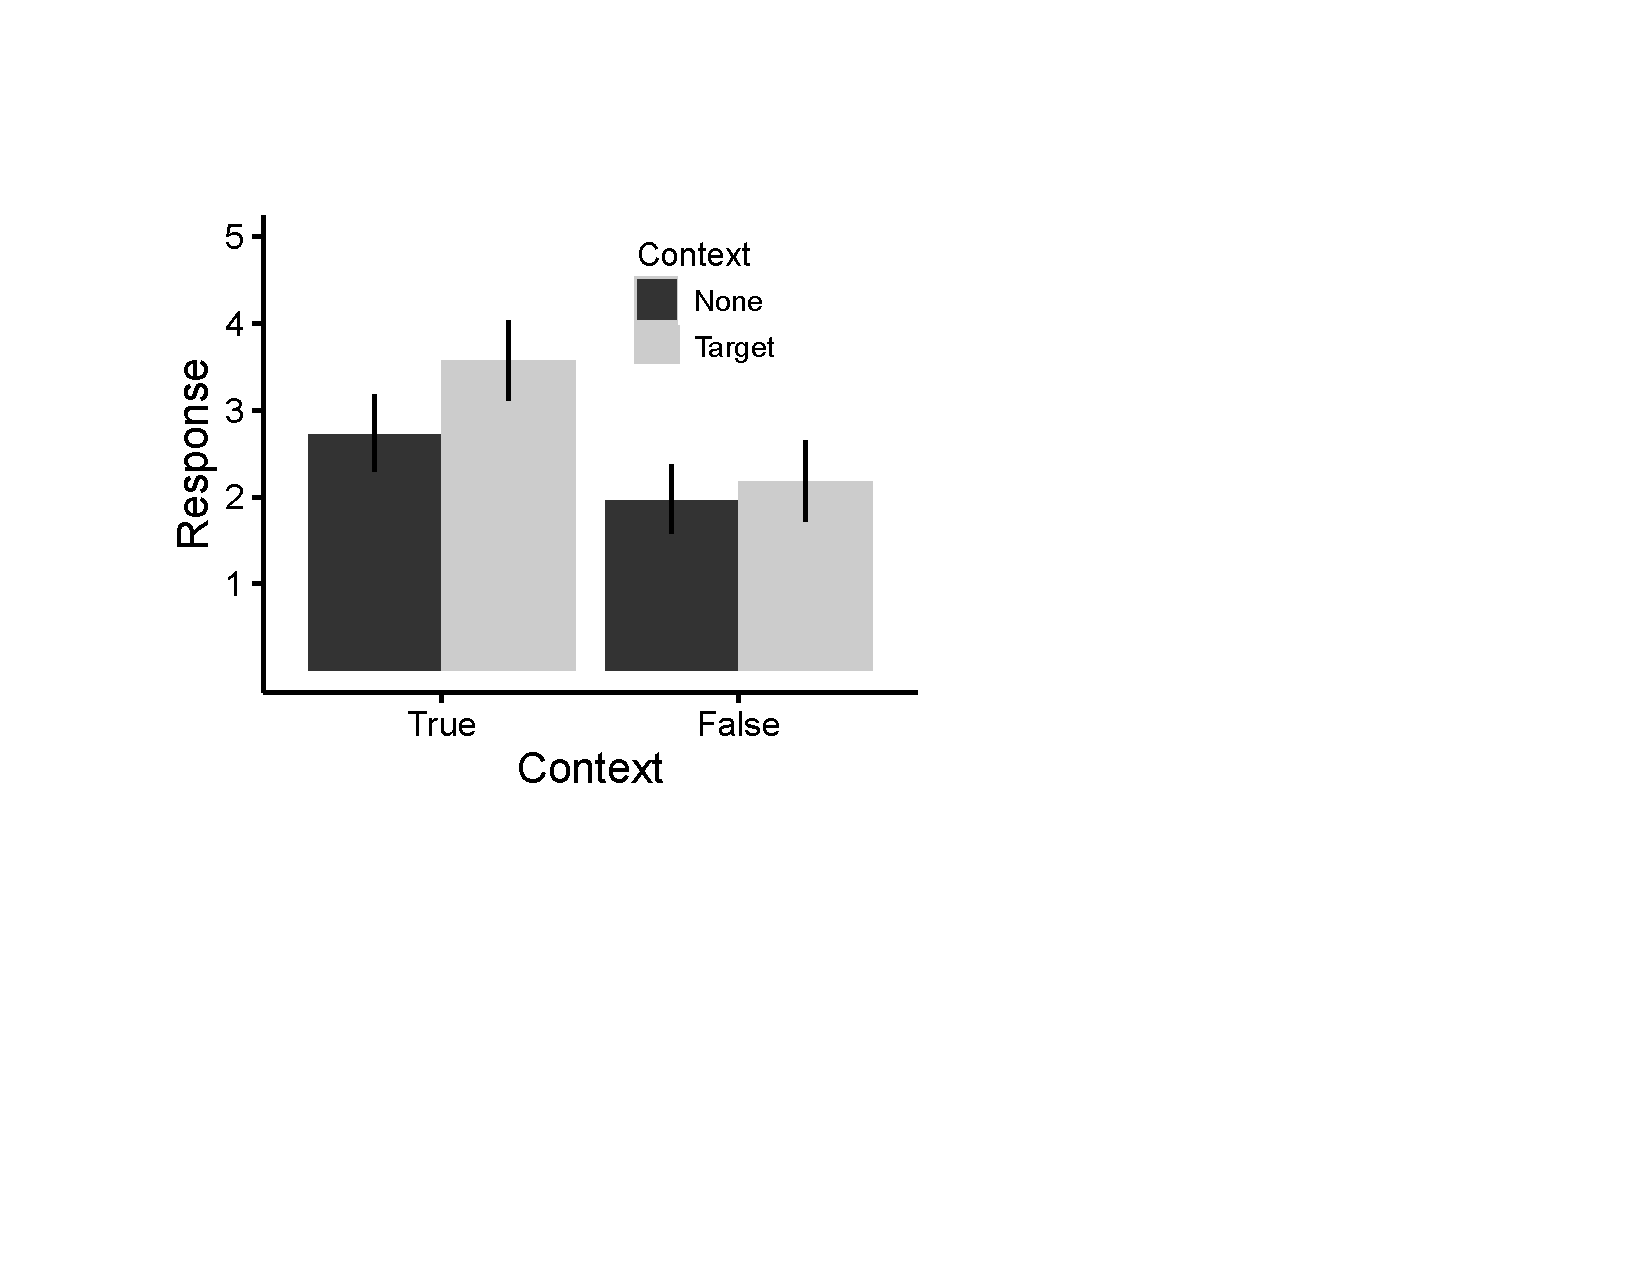
\includegraphics[width=3.5in]{figures/childmeans.pdf}
\caption{\label{fig:childmeans} Children's mean ratings for true and false negative sentences in the none and target contexts in Experiment 2. Responses to true negatives are shown on the left, and responses to false negatives are shown on the right. Trials with a none context are shown in black, and trials with a target context are shown in gray. Error bars show 95\% confidence intervals.}
\end{center}
\end{figure}

We fit a linear mixed-effects model to test the effects of context and truth value on children's negative sentence ratings.\footnote{ The model specification was as follows: \texttt{rating $\sim$ context~$\times$~truth + (1~\textbar~subject) + (1~\textbar~item)}}  Because children were trained, with feedback, on positive sentences to familiarize them with the scale, and exclusion criteria was based on children's performance on positive sentences, we focus on children's responses to negative sentences in our analyses. Results of this model can be seen in Table \ref{tab:s3.1}. A linear mixed-effects model that included children's age group did not yield a significant effect of age (three-year-olds vs. four-year-olds), and did not significantly improve model fit ($\chi ^{2}(4) = 2.86$, $p=.58$).

Children rated true negative sentences significantly higher than false negative sentences ($\beta= -1.07$, $p< .001$), indicating that they correctly perceived and processed the negation and recognized that false negative sentences were incorrect. We also found a main effect of context, with children rating sentences in the none condition significantly lower than sentences in the target condition ($\beta= -0.55$, $p< .05$). This supports our hypothesis that children are sensitive to the contexts of negation, and that children's past difficulties responding to negative sentences is due to the context in which these sentences were, rather than a difficulty in processing negation. The interaction between truth value and context condition was not significant ($\beta= 0.61$, $p=.2$).

\begin{table}[t]
\caption{\label{tab:s3.1} Coefficient estimates from a mixed-effects model predicting negative sentence ratings in Experiment 3.}
\begin{center}
\small\addtolength{\tabcolsep}{-5pt}
\begin{tabular}{rrrr}
 \hline
 & Coefficient & Std. err. & t value \\
 \hline
(Intercept) & 2.61 & 0.11 & 23.46 \\
 Context & -0.55 & 0.22 & -2.46 \\
 Truth Value & -1.07 & 0.24 & -4.48 \\
 Context$\times$Truth Value & 0.61 & 0.48 & 1.28 \\
  \hline
\end{tabular}
\end{center}
\end{table}

%I cut this, because context is significant in the above model so these additional analyses seem redundant?
%Although the above model did not yield a significant interaction between truth condition and context, a histogram of children's responses to true negative sentences suggests a striking difference in the distribution of responses to true negative sentences in the target vs. the none condition (Figure \ref{fig:histograms}). To test whether this difference is significant, we fit a linear mixed-effects model testing the effect of context on children's ratings for only true negative sentences. This post-hoc analysis yielded a significant effect of context on children's ratings for true negative sentences (RESULTS), suggesting that children rated true negative sentences higher in the target context than the none context. A post-hoc t-test comparing children's ratings to true negatives in the two context conditions yielded similarly significant results, RESULTS.

%Figure \ref{fig:histograms} shows histograms of three-year-olds' and four-year-olds' responses to true negative trials, as well as the mean responses to true negative trials in each context condition. Both three- and four-year-olds were significantly more likely to rate a true negative sentence as ``very good'' in the target context, and were significantly more likely to rate a true negative sentence as ``very silly / a mistake'' in the none context. This effect of context, however, appears to be more pronounced amongst four-year-olds compared to three-year-olds. To examine the effect of context on true negative sentence ratings in each age group, we separately compared each age groups' responses to true negative sentences in the target context and the none context. A two-sample t-test showed that the difference between true negative ratings in the target context and the none context was not significant for three-year-olds ($t(32) = -1.56$, $p=0.13$), but was significant for four-year-olds ($t(32) = -2.09$, $p<.05$), indicating that four-year-olds rated true negative sentences significantly lower in the none context compared to the target context.


\begin{figure}
\begin{center}
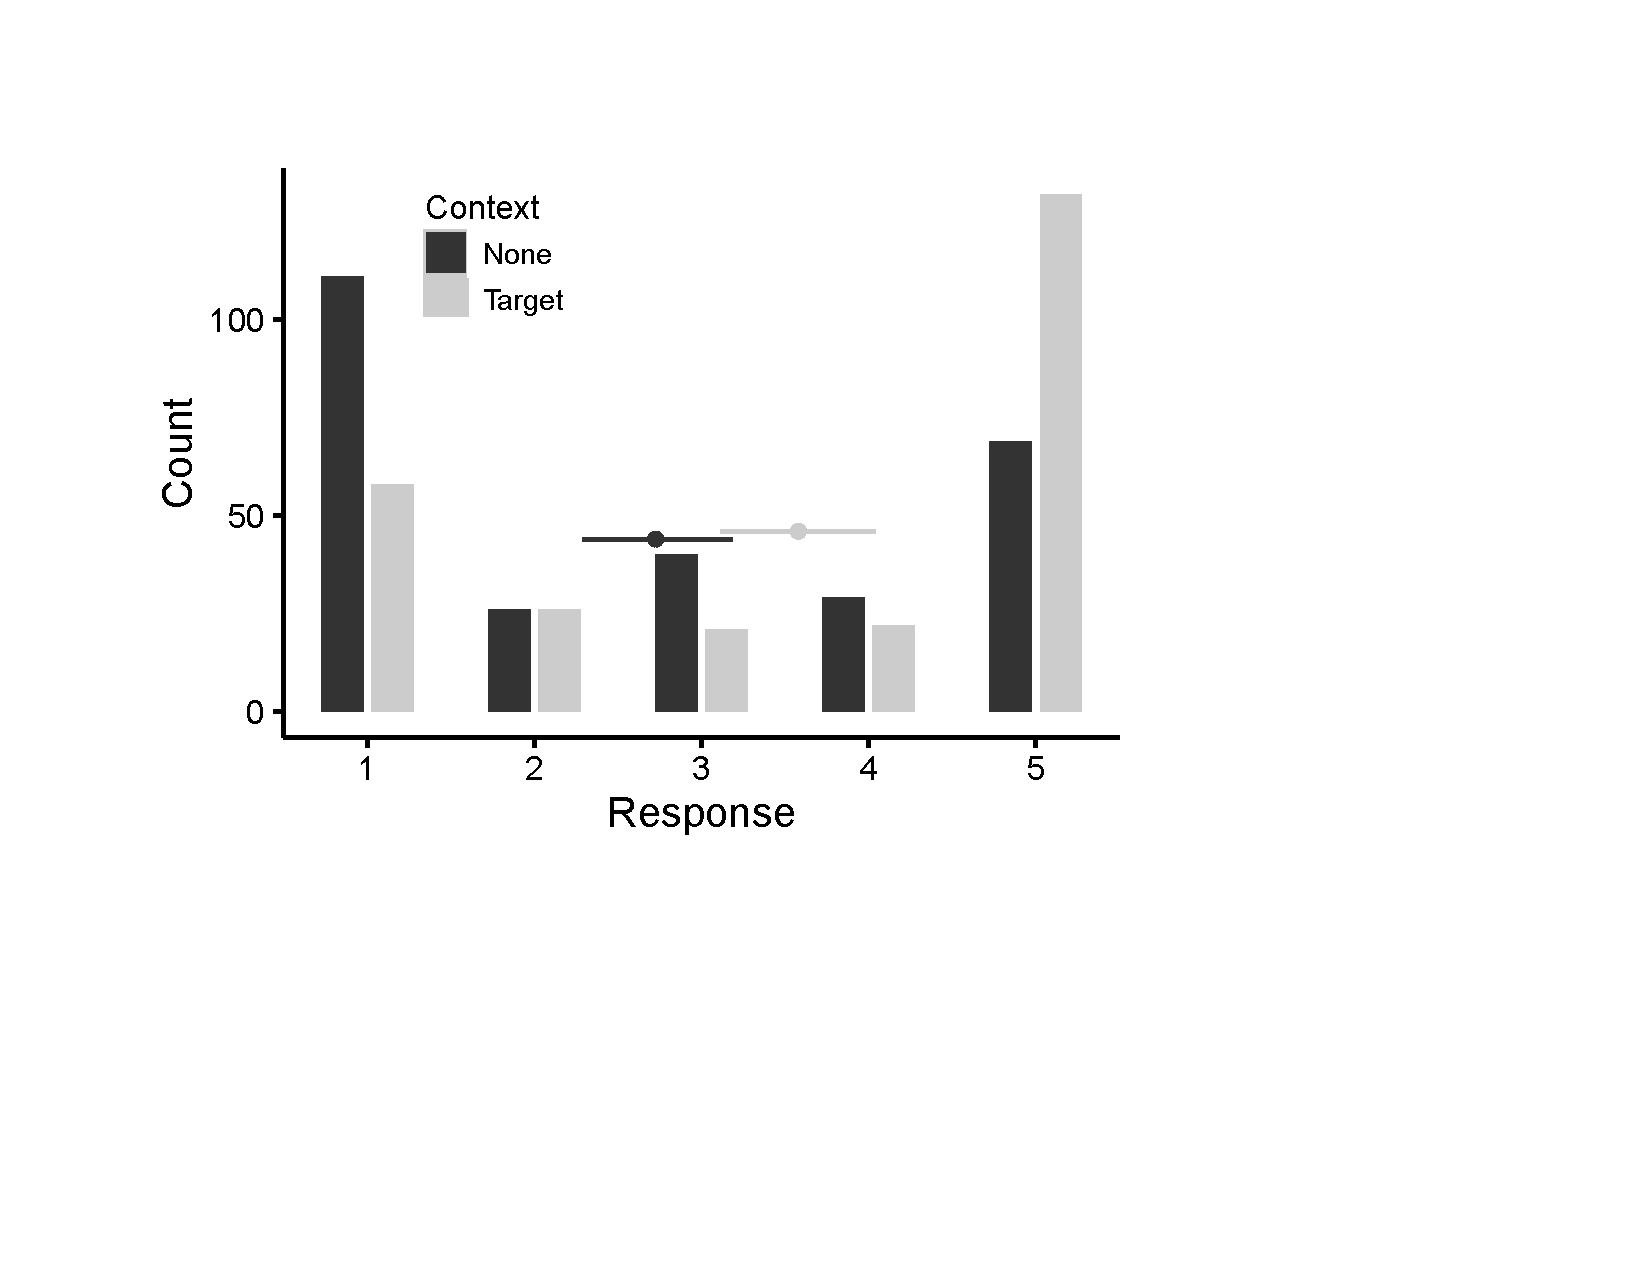
\includegraphics[width=4in]{figures/hist_all.pdf}
\caption{\label{fig:histograms} Histograms of children's responses to true negative trials in the target context and the none context. Black bars represent responses in the none context, and gray bars represent responses in the target context. Points represent the mean response in each group, and horizontal error bars show 95\% confidence intervals.}
\end{center}
\end{figure}

These results suggest that children are sensitive to the contexts in which they hear a negative sentence. Similar to adults, children found negative sentences to be ``silly'' or a mistake when they were produced without any contextual support, but were more likely to say that the same sentences were ``good'' in a supportive context. In addition, children had no difficulty with false negative sentences, suggesting that their performance in response to true negative sentences is not due to confusion about how negation works or difficulty processing negation, but rather a sensitivity to the pragmatics of negation. These results are consistent with the hypothesis that children's responses to these sentences is due to their sensitivity to pragmatics, rather than a difficulty specific to negation.


\section{General Discussion}

Past work suggests that both children and adults struggle to comprehend and process negative sentences \cite<e.g.>{hclark1972, kim1985}.  We propose that this difficulty is due to general pragmatic principles that govern all communication, rather than difficulties specific to negation.  Our results support this hypothesis: The types of contexts that supported the processing of negative sentences in previous work led to higher felicity ratings from both adults and children in our studies.  We argue that pragmatic informativeness is the mechanism by which context influences the felicity of negative sentences, and that children are sensitive to the ways that context influences informativeness.

In our experiments, we found that contextual differences led to significantly different pragmatic judgments for otherwise identical true grammatical negative sentences. What is it about the context of negative sentences that elicits these effects? One hypothesis is that felicity ratings are influenced by the \emph{informativeness} of true negative sentences. According to theories of pragmatics, speakers should produce sentences that are appropriately informative based on the context. In a context where most characters have apples and one does not, it is informative to mention the latter character's lack of apples, because this feature is unique to the character being described. In our data, the negative sentences that received the lowest felicity ratings for both adults and children were alternative negations in a none context. On these trials, participants saw e.g., three characters with nothing, and a character with a cat (see Figure \ref{fig:trial}). The sentence ``Abby doesn't have an apple'' referred to the character with a cat. Although this sentence is true, it sounds very odd: Why is the speaker talking about Abby's lack of apples, which is true of everyone in the context, instead of mentioning the cat? Compare this example to nonexistence negation in a target context, which elicited the highest ratings for adult participants: Three characters have apples, and Abby has nothing. Here, the same sentence sounds  natural, because Abby's lack of apples is unique, and there is little else to say about her. In this latter context, producing a negative sentence is reasonable and perhaps even expected.

Our findings support our hypothesis that children's difficulty comprehending negation is due to the infelicity of negative sentences out of context.  Children's responses to negative sentences in the none context replicate past findings \cite{kim1985}: The majority of children said that the true negative sentences were ``silly'' or ``a mistake,'' despite the fact that the sentences were true. In contexts where all of the context characters possessed the negated item, however, children's behavior shifted substantially, with the majority of children rating the true sentences as ``good.'' These findings suggest that children's past failures on similar comprehension tasks are likely due to the infelicity of pragmatically unsupported negation. Instead of seeing children's responses as incorrect, we can instead interpret them as felicity judgments: Children in the none context are saying that the sentence is wrong or a mistake not because it is \emph{false}, but because it is \emph{infelicitous}.

In addition, children's performance on this task suggests a sensitivity to the contexts of communication more generally. According to Neo-Gricean theories of communication, speakers should produce sentences that are maximally informative and relevant given the context. In our experiment, the none context was both uninformative and irrelevant. Children's differential responses to true negative sentences in these two contexts suggests that children are aware of these communicative principles, and expect speakers (and puppets) to abide by them.

We did not find evidence for developmental change in children's responses between three- and four-year-olds. Although the difference between contexts was not statistically significant for three-year-olds, children of both age groups rated true negative sentences higher in the target context compared to the none context. Based on the prior evidence from the negation acquisition literature, this finding is surprising: Past studies of children's comprehension of denial and nonexistence negation suggest that two- and three- year olds struggle to respond correctly to true negative sentences, but improve by age four or five \cite{kim1985, nordmeyer2014b}. If, however, children's performance on tests of negation comprehension is pragmatic in nature, it's possible that even the youngest children in our sample already have the pragmatic abilities to be sensitive to this difference in context. Due to the metacognitive demands of the felicity judgment task, however, a different paradigm would likely need to be used to test younger children's sensitivity to the contexts of negative sentences.

Past work on children's processing of negation suggests that some experimental paradigms may involve processing demands that make it difficult for children to respond correctly to negative sentences. For example, in \citeNP{nordmeyer2014b}, children (especially 3-year-olds) in a gaze-following task struggled to look at the correct referent of a negative sentence, especially when the negative sentence referred to nonexistence. One explanation is that when children are asked to ``Find the boy with no apples,'' the referent of the sentence is much less interesting in a nonexistence context (because the referent is a boy with nothing, and the distractor is a boy with apples); reaction times in that study suggest that three-year-olds did shift their gaze to the correct picture initially, but quickly returned to looking at the more interesting picture. Both three- and four-year-olds  were more successful in an alternative negation context, supporting this interpretation \cite{nordmeyer2014b}. In the present study we did not test children on nonexistence negation; it is possible that these processing demands would have made the task more difficult. One advantage to this paradigm, however, is that children do not need to maintain their gaze on a less interesting character in order indicate their response, which may have reduced these demands. The fact that adults' felicity judgments did not show an interaction between context and negation type lead us to believe that children would still be sensitive to the effect of context if tested on nonexistence negation, although it is possible they would find the task somewhat more difficult due to these processing demands.

One consistent finding for both adults and children was the greater effect of context on true negative compared to false negative sentences. Our primary focus was on true negative sentences, because these have been shown to be influenced by context in the past \cite{wason1965, glenberg1999, nordmeyer2014b} and are the most difficult sentence type in classic sentence verification tasks \cite{hclark1972}. It is striking to note, however, that for both adults and children we found significant effects of context on the evaluation of true negative sentences, but no effect of context on the evaluation of false negative sentences. One possibility is that this finding reflects a floor effect, and that participants rate false sentences at the lowest end of a felicity scale by default. Another possibility, however, is that hearing a false sentence is such a gross violation of the Cooperative Principle that speakers don't consider additional violations, such as an uninformative and irrelevant false sentence.

Most Neo-Gricean theories of communication are based on ideas about how real-time, face-to-face communication works. In the real world, the types of contexts that negative sentences occur in are rich and varied. Many kinds of information might influence the felicity of a negative sentence: Your real-world knowledge, the previous utterances in a conversation, the joint activity that you are engaged in with another speaker, etc. In our experiments, we used stripped-down contexts with little to no interaction between the ``speaker'' and the participant. Even in Experiment 2, although a puppet ``spoke'' the words, children were told to rate the puppet's utterance on the iPad rather than speaking to the puppet directly, making this task very different from natural conversation. Despite this unnatural communicative setting, we found consistent evidence that both adults and children were sensitive to the context that a negative sentence occurred in. These results are consistent with past data on the effects of a wider range of contexts on the of processing of negative sentences \cite{clark1976, wason1965, glenberg1999, nieuwland2008, dale2011, nordmeyer2014}. Our findings suggest that the pragmatics of language use are embedded in all contexts in which we use language, and are not merely an optional feature of face-to-face communication.

According to Grice's Cooperative Principle, speakers should produce utterances that are informative with respect to their intended meaning. If listeners expect speakers to abide by this principle, they should find uninformative sentences infelicitous. Our results support this view of communication: Negative sentences that were more informative (and therefore more likely to be produced by a speaker) were given higher felicity ratings. These data suggest that general pragmatic factors, rather than some specific quirk of negation, can explain the felicity of negative sentences in context.

\subsection{Acknowledgments}
This work supported by the NSF GRFP. Portions of this work were presented in \citeNP{nordmeyer2014c} and \citeNP{nordmeyer2015}.

\bibliographystyle{apacite}

\setlength{\bibleftmargin}{.125in}
\setlength{\bibindent}{-\bibleftmargin}

\bibliography{negation}

\newpage
\theappendix

\section{Appendix A: Mean felicity ratings in Experiment 1}\label{appendix:exp1}

\begin{table}[h!]
\caption{\label{tab:m1} Mean felicity rating for different trial types in Experiment 1, based on ratings given on a 7-point scale.}
\begin{center}
\small\addtolength{\tabcolsep}{-5pt}
\begin{tabular}{llllrr}
 \hline
 Context & Sentence type & Truth Value & Referent Type & Mean & Std. Dev. \\
 \hline
 None & Positive & True & Target item & 6.51 & 0.89\\
 None & Positive & False & Nothing & 2.51 & 1.94\\
 None & Positive & False & Alternative item & 2.04 & 1.82\\
 None & Negative (``doesn't have'') & True & Nothing & 5.29 & 1.44\\
 None & Negative (``doesn't have'') & True & Alternative item & 4.83 & 1.92\\
 None & Negative (``doesn't have'') & False & Target item & 2.00 & 1.64\\
 None & Negative (``has no'') & True & Nothing & 4.78 & 1.68\\
 None & Negative (``has no'') & True & Alternative item & 4.15 & 1.78\\
 None & Negative (``has no'') & False & Target item & 1.40 & 0.77\\
 Target & Positive & True & Target item & 6.42 & 0.76\\
 Target& Positive & False & Nothing & 1.88 & 1.47\\
 Target & Positive & False & Alternative item & 1.83 & 1.73\\
 Target & Negative (``doesn't have'') & True & Nothing & 6.34 & 1.11\\
 Target & Negative (``doesn't have'') & True & Alternative item & 5.74 & 1.41\\
 Target & Negative (``doesn't have'') & False & Target item & 1.89 & 1.60\\
 Target & Negative (``has no'') & True & Nothing & 5.61 & 1.51\\
 Target & Negative (``has no'') & True & Alternative item & 4.96 & 1.41\\
 Target & Negative (``has no'') & False & Target item & 1.58 & 0.99\\
  \hline
\end{tabular}
\end{center}
\end{table}

\newpage

\section{Appendix B: Mean felicity ratings in Experiment 2}\label{appendix:exp2}

\begin{table}[h!]
\caption{\label{tab:m3} Children's mean felicity rating for different trial types in Experiment 2, based on ratings given on a 5-point scale.}
\begin{center}
\small\addtolength{\tabcolsep}{-5pt}
\begin{tabular}{lllrr}
 \hline
 Context & Sentence type & Truth Value & Mean & Std. Dev. \\
 \hline
 None & Positive & True & 4.59 & 0.70\\
 None & Positive & False & 1.77 & 1.04\\
 None & Negative & True & 2.72 & 1.44 \\
 None & Negative & False & 1.96 &1.23 \\
 Target & Positive & True & 4.61 & 0.57\\
 Target & Positive & False & 1.48 & 0.83 \\
 Target & Negative & True & 3.58 & 1.37 \\
 Target & Negative & False & 2.18 & 1.38\\
  \hline
\end{tabular}
\end{center}
\end{table}

\end{document}
